\documentclass[11pt]{aghdpl}
% \documentclass[en,11pt]{aghdpl}  % praca w języku angielskim

% Lista wszystkich języków stanowiących języki pozycji bibliograficznych użytych w pracy.
% (Zgodnie z zasadami tworzenia bibliografii każda pozycja powinna zostać utworzona zgodnie z zasadami języka, w którym dana publikacja została napisana.)
\usepackage[english,polish]{babel}

%%% fix for \lll
\let\babellll\lll
\let\lll\relax

% Użyj polskiego łamania wyrazów (zamiast domyślnego angielskiego).
\usepackage{polski}

\usepackage[utf8]{inputenc}

\newcommand*{\captionsource}[2]{%
  \caption[{#1}]{%
    #1%
    \\\hspace{\linewidth}%
    \textbf{Żródło:} #2%
  }%
}

% dodatkowe pakiety

\usepackage{mathtools}
\usepackage{amsfonts}
\usepackage{amsmath}
\usepackage{amsthm}
\usepackage{amssymb}
\usepackage{float}

\numberwithin{equation}{section}

% --- < bibliografia > ---

\usepackage[
style=numeric,
sorting=none,
%
% Zastosuj styl wpisu bibliograficznego właściwy językowi publikacji.
language=autobib,
autolang=other,
% Zapisuj datę dostępu do strony WWW w formacie RRRR-MM-DD.
urldate=iso8601,
% Nie dodawaj numerów stron, na których występuje cytowanie.
backref=false,
% Podawaj ISBN.
isbn=true,
% Nie podawaj URL-i, o ile nie jest to konieczne.
url=false,
%
% Ustawienia związane z polskimi normami dla bibliografii.
maxbibnames=3,
% Jeżeli używamy BibTeXa:
backend=bibtex
]{biblatex}

\usepackage{csquotes}
% Ponieważ `csquotes` nie posiada polskiego stylu, można skorzystać z mocno zbliżonego stylu chorwackiego.
\DeclareQuoteAlias{croatian}{polish}

\addbibresource{bibliografia.bib}

% Nie wyświetlaj wybranych pól.
%\AtEveryBibitem{\clearfield{note}}


% ------------------------
% --- < listingi > ---

% Użyj czcionki kroju Courier.
\usepackage{courier}

\usepackage{listings}
\lstloadlanguages{TeX}

\lstset{
	literate={ą}{{\k{a}}}1
           {ć}{{\'c}}1
           {ę}{{\k{e}}}1
           {ó}{{\'o}}1
           {ń}{{\'n}}1
           {ł}{{\l{}}}1
           {ś}{{\'s}}1
           {ź}{{\'z}}1
           {ż}{{\.z}}1
           {Ą}{{\k{A}}}1
           {Ć}{{\'C}}1
           {Ę}{{\k{E}}}1
           {Ó}{{\'O}}1
           {Ń}{{\'N}}1
           {Ł}{{\L{}}}1
           {Ś}{{\'S}}1
           {Ź}{{\'Z}}1
           {Ż}{{\.Z}}1,
	basicstyle=\footnotesize\ttfamily,
}

% ------------------------

\AtBeginDocument{
	\renewcommand{\tablename}{Tabela}
	\renewcommand{\figurename}{Rys.}
}

% ------------------------
% --- < tabele > ---

\usepackage{array}
\usepackage{tabularx}
\usepackage{multirow}
\usepackage{booktabs}
\usepackage{makecell}
\usepackage[flushleft]{threeparttable}

% defines the X column to use m (\parbox[c]) instead of p (`parbox[t]`)
\newcolumntype{C}[1]{>{\hsize=#1\hsize\centering\arraybackslash}X}


%---------------------------------------------------------------------------

\author{Marcin Kowalczyk}
\shortauthor{M. Kowalczyk}

\titlePL{System wizyjny śledzący obiekty wykorzystujący ruchomą kamerę zrealizowany w oparciu o heterogeniczny układ Zynq.}
\titleEN{An object tracking vision system using a moving camera implemented in a Zynq heterogeneous device.}


\shorttitlePL{System wizyjny realizujący śledzenie z ruchomą kamerą.}
\shorttitleEN{An object tracking vision system with moving camera.}

\thesistype{Praca dyplomowa inżynierska}

\supervisor{dr inż. Tomasz Kryjak}

\degreeprogramme{Automatyka i Robotyka}

\date{2016}

\department{Katedra Automatyki i Inżynierii Biomedycznej}

\faculty{Wydział Elektrotechniki, Automatyki,\protect\\[-1mm] Informatyki i Inżynierii Biomedycznej}

\acknowledgements{Serdecznie dziękuję \dots tu ciąg dalszych podziękowań np. dla promotora, żony, sąsiada itp.}


\setlength{\cftsecnumwidth}{10mm}

%---------------------------------------------------------------------------
\setcounter{secnumdepth}{4}
\brokenpenalty=10000\relax

\begin{document}

\titlepages

% Ponowne zdefiniowanie stylu `plain`, aby usunąć numer strony z pierwszej strony spisu treści i poszczególnych rozdziałów.
\fancypagestyle{plain}
{
	% Usuń nagłówek i stopkę
	\fancyhf{}
	% Usuń linie.
	\renewcommand{\headrulewidth}{0pt}
	\renewcommand{\footrulewidth}{0pt}
}

\setcounter{tocdepth}{2}
\tableofcontents
\clearpage

\chapter{Wstęp}
\label{cha:wstep}

\section{Cel pracy}
\label{sec:celpracy}

Celem pracy jest stworzenie demonstratora systemu wizyjnego do śledzenia obiektów, przy czym zakłada się, że kamera zamontowana jest na głowicy obrotowej. Praca inżynierska obejmuje skompletowanie, we współpracy z opiekunem, stanowiska testowego składającego się z głowicy ruchomej, kamery, platformy obliczeniowej oraz wskaźnika. Należy przeprowadzić analizę oraz weryfikację różnych koncepcji śledzenia, biorąc pod uwagę skuteczność oraz możliwość implementacji sprzętowej lub sprzętowo-programowej. Wybrane rozwiązanie zostało zaimplementowane, uruchomione i przetestowane w sprzęcie. Wyjście z modułu śledzenia stanowi podstawę do wypracowania pozycjonowania głowicy obrotowej, takiego, aby utrzymać obiekt w środku kadru oraz oznaczyć go wskaźnikiem.

\section{Wprowadzenie}
\label{sec:wprowadzenie}

Automatyczne śledzenie z pomocą kamery jest wykorzystywane m.in. w zagadnieniach związanych z bezpieczeństwem, inwigilacją lub w zastosowaniach wojskowych. Jest ściśle powiązane z wykrywaniem oraz identyfikacją obiektów. Świadczy to o złożoności tego zagadnienia. Śledzenie różni się od innych algorytmów przetwarzania obrazów głównie tym, że musimy wykorzystywać informacje pochodzące z więcej niż jednego kadru. Uwydatnia się to szczególnie, kiedy kamera rejestruje kilka obiektów podobnych do śledzonego. Jeśli zadaniem jest obserwacja jednego konkretnego obiektu, to aby go wyróżnić musimy wykorzystać położenie śledzonego obiektu w poprzednich ramkach \cite{VT}. Znaczące problemy w śledzeniu obiektów mogą być spowodowane zmianą orientacji celu oraz dużą jego szybkością w porównaniu do częstotliwości rejestrowania klatek. W przypadku kamery umieszczonej na głowicy błędy mogą być dodatkowo spowodowane rozmyciem obrazu w trakcie poruszania układu. Istnieją liczne algorytmy służące śledzeniu elementu na obrazach z kamery. Są to m.in:
\begin{itemize}
\item{Śledzenie przez detekcję}
\item{Mean-shift}
\item{Filtr cząsteczkowy}
\item{KLT}
\end{itemize}
Algorytmy te zostaną dokładniej omówione w kolejnym rozdziale pracy.

\section{Zawartość pracy}
\label{sec:zawartoscpracy}

W rozdziale \dots
\chapter{Algorytmy}
\label{cha:algorytmy}

W rozdziale tym omówione zostaną algorytmy śledzenia. Rozważymy również możliwość oraz skuteczność ich implementacji sprzętowej i sprzętowo-programowej.

\section{Śledzenie przez detekcję}
\label{sec:sledzenieprzezdetekcje}

Jest to najłatwiejszy możliwy algorytm śledzenia. Polega on na detekcji obiektu i określeniu jego położenia (np. poprzez wyznaczenie środka ciężkości). Algorytm ten jest efektywny tylko, gdy w kadrze znajduje się maksymalnie jeden wyznaczony obiekt. Ograniczenie to możemy obejść przez zastosowanie dodatkowo algorytmu indeksacji. Wtedy musimy zdecydować który z wyznaczonych obiektów jest tym właściwym. Możemy np. śledzić element znajdujący się najbliżej (mający największą powierzchnię w kadrze). Efektywność implementacji programowo-sprzętowej zależy w większości od wykorzystanego algorytmu detekcji, i/lub segmentacji. Algorytm detekcji na podstawie koloru będzie łatwy i szybki do zaimplementowania, a algorytm bazujący na współczynnikach kształtu  wymagać będzie dużo więcej pracy i zasobów.

\section{Mean-shift}
\label{sec:meanshift}

Algorytm ten bazuje na statystycznej metodzie poszukiwania lokalnego maksimum rozkładu prawdopodobieństwa. Polega on na wyznaczeniu maksymalnej wartości prawdopodobieństwa w aktualnym oknie wokół punktu startowego. W celu zastosowania tego algorytmu do śledzenia obiektu należy przedstawić obraz jako rozkład prawdopodobieństwa. W tym celu każdemu pikselowi przypisuje się wartość prawdopodobieństwa. Można to zrobić np. na podstawie koloru, przypisując kolorom wartość prawdopodobieństwa, lub histogramu, porównując histogram otoczenia piksela z histogramem obiektu \cite{CMS}. Jeśli prawdopodobieństwo obliczone zostaje tylko na podstawie koloru, dobre wyniki można uzyskać, gdy \cite{CMS}:
\begin{itemize}
\item Obiekt ma jednolitą barwę.
\item Występują bardzo małe zmiany oświetlenia.
\item W kadrze nie ma obiektów podobnych do śledzonego.
\item Kolor tła znacznie różni się od koloru obiektu.
\item Obiekt nie zostaje całkowicie zasłonięty.
\end{itemize}
\paragraph*{}
Algorytm ten ma następujący przebieg:
\begin{enumerate}
\item Wybierz rozmiar okna.
\item Wybierz początkowe położenie(środek) okna.
\item Wyznacz położenie maksimum wartości prawdopodobieństwa w oknie.
\item Przesuń okno, aby wyznaczone maksimum było jego środkiem.
\item Powtarzaj kroki 3 i 4, aż algorytm będzie zbieżny.
\end{enumerate}
\paragraph*{}
Punktem startowym dla każdego kolejnego obrazu z kamery jest pozycja obiektu w poprzednim obrazie. Poszukiwanie maksymalnej wartości prawdopodobieństwa odbywa się w następujący sposób:
\begin{itemize}
\item Obliczamy moment zerowy.
\begin{equation}
M_{00}=\sum\limits_{x}\sum\limits_{y}l(x,y)
\end{equation}
\item Obliczamy moment pierwszy dla osi poziomej.
\begin{equation}
M_{10}=\sum\limits_{x}\sum\limits_{y}x \cdot l(x,y)
\end{equation}
\item Obliczamy moment pierwszy dla osi pionowej.
\begin{equation}
M_{01}=\sum\limits_{x}\sum\limits_{y}y \cdot l(x,y)
\end{equation}
\item Obliczamy środek rozkładu prawdopodobieństwa w danym oknie.
\begin{equation}
x_c=\frac{M_{10}}{M_{00}}
\end{equation}
\begin{equation}
y_c=\frac{M_{01}}{M_{00}}
\end{equation}
\end{itemize}
Gdzie \(l(x,y)\) jest wartością prawdopodobieństwa dla piksela \((x,y)\)\cite{BCV}.

%\paragraph*{}
%Można wykorzystać przykładowe jądra:
%\begin{itemize}
%\item Płaskie
%\[K(x)=\begin{cases}1 & \text{dla } x \leqslant R \\ 0 & \text{dla } x>R \end{cases}\]
%\item Gaussowskie
%\[K(x)=\frac{1}{2\pi}\mathrm{e}^{-\frac{1}{2} \cdot |x|^2}\]
%\end{itemize}
%\paragraph*{}
%Dla zestawu \(n\) punktów w 2-wymiarowej przestrzeni estymacja gęstości jądra z jądrem K(x) i promieniem %#\(h\) wynosi:
%#\[f_K(x)=\frac{1}{nh^2} \cdot \sum\limits_{i=1}^{n}K(\frac{x-x_i}{h})\]

\section{Filtr cząsteczkowy}
\label{sec:filtrczasteczkowy}

Filtr cząsteczkowy inaczej nazywany jest sekwencyjną metodą Monte Carlo. Punktem startowym algorytmów tego typu jest model obiektu w postaci równań stanu \cite{Mukhtar}:
\begin{equation}
\label{eq:PF_state}
x_k=Ax_{k-1}+Bu_k+w_{k-1}
\end{equation}
\begin{equation}
y_k=Cx_k+v_k
\end{equation}
\(x_k\) jest ukrytym, prawdziwym stanem obiektu.\newline
\(y_k\) jest obserwowanym stanem obiektu.\newline
\(w_{k-1}\) jest zmienną losową o rozkładzie normalnym reprezentującą szum przetwarzania.\newline
\(v_k\) jest zmienną losową o rozkładzie normalnym reprezentującą szum pomiarowy.\newline
%Jeśli obiekt porusza się ze stałą prędkością, przyjąć należy następujące macierze \(A\) i \(B\):
%\begin{equation}
%A=2 \cdot I
%\end{equation}
%\begin{equation}
%B=-I
%\end{equation}

\paragraph*{}
Algorytm korzysta z wyprowadzonej z twierdzenia Bayesa rekurencyjnej zależności:
\begin{equation}
p(x_{k+1}|y_{0:k+1}) \propto p(y_{k+1}|x_{k+1}) \int\limits_{x_k} p(x_{k+1}|x_k)p(x_k|y_{0:k})dx_k
\end{equation}
\(x_{0:k}\) oznacza wektor \((x_0,\dots,x_k)\).
Powyższy wzór opisuje rozkład prawdopodobieństwa, zmiennej \(x_{k+1}\), pod warunkiem, że znane są dotychczasowe pomiary \(y_{0:k+1}\). Wartość oczekiwana tego rozkład przyjmowana jest jako wynik zadania śledzenia. W opisywanym algorytmie równanie to rozwiązywane jest metodą Monte Carlo, która skomplikowane problemy przybliża za pomocą zbioru losowo rozmieszczonych cząstek. W omawianym przypadku przybliżaną wielkością jest prawdopodobieństwo \(p(x_{k+1}|y_{0:k+1})\). Cząsteczki reprezentują możliwe położenia śledzonego obiektu \cite{Meresinski}.

\paragraph*{}
Następnie należy każdej cząsteczce przypisać wagę, która reprezentuje prawdopodobieństwo \(p(y_{k+1}|x_{k+1})\). Może być określona np. w następujący sposób \cite{Meresinski}:
\begin{equation}
w_i=ke^{-\Lambda D^2}
\end{equation}
\(k\) jest stałą normalizującą sumę wag.
\(\Lambda\) jest parametrem algorytmu.
\(D\) jest dystansem.

Najczęściej stosownym dystansem jest podobieństwo histogramu cząsteczki z histogramem bazowym obiektu. Pozycja obiektu wyznaczana jest następująco:
\begin{equation}
\label{eq:PF_polozenie}
x_{k+1}=\sum\limits_{i=1}^{M} w_{i,k+1} \cdot x_{i,k+1}
\end{equation}

Ostatnim etapem jest powielenie cząstek. Losowanych jest M cząstek z prawdopodobieństwem określonym przez wyliczone wagi (cząstka może być wylosowana więcej niż jeden raz). Następnie są one rozrzucane zgodnie z równaniem \ref{eq:PF_state}. Jest to etap predykcji. W wyniku tego działania większość cząstek znowu znajduje się w otoczeniu śledzonego obiektu.

\paragraph*{}
Algorytm ma następujący przebieg \cite{Meresinski}:
\begin{enumerate}
\item Wyznaczenie histogramu śledzonego obiektu.
\item Rozmieszczenie cząstek wokół początkowego położenia obiektu zgodnie z wybranym rozkładem (najczęściej normalnym).
\item Etap przewidywania. Przesunięcie cząstek zgodnie z równaniami stanu \ref{eq:PF_state}.
\item Obliczenie histogramu w otoczeniu każdej cząstki.
\item Obliczenie wagi każdej cząstki.
\item Obliczenie najbardziej prawdopodobnego położenia obiektu zgodnie z równaniem \ref{eq:PF_polozenie}.
\item Powielenie cząstek.
\end{enumerate}

\section{KLT}
\label{sec:klt}
Algorytm opisany przez Kanade'a, Lucas'a i Tomasi'a może posłużyć do śledzenie obiektu na obrazie w skali szarości. Polega on na poszukiwaniu najlepszego dopasowania obrazu referencyjnego \(T(x)\) do aktualnej ramki otrzymanej z kamery \(I(x)\) \cite{TSK}. Obrazy te są przesuwane względem siebie o wektor \(p\):
\begin{equation}
W(x,p)=
	\begin{bmatrix}
	x_1+p_1 \\
	x_2+p_2
	\end{bmatrix}
\end{equation}
Poszukiwane jest więc minimum następującej funkcji:
\begin{equation}
f(x,p)=\sum\limits_{x}((I(W(x,p))-T(x))^2
\end{equation}
Zakłada się, że początkowa wartość przesunięcia \(p\) jest znana, a poszukiwana jest najlepsza modyfikacja tego przesunięcia \(\Delta p\).
\begin{equation}
f(x,\Delta p)=\sum\limits_{x}((I(W(x,p+\Delta p))-T(x))^2
\end{equation}
Po znalezieniu optymalnego przesunięcia \(\Delta p\) aktualizowana jest wartość przesunięcia początkowego:
\begin{equation}
p \leftarrow p+\Delta p
\end{equation}
\paragraph*{}
Funkcja \(I(x,p+\Delta p)\) linearyzowana jest w otoczeniu punktu \((x,p)\) ze względu na \(\Delta p\) poprzez rozwinięcie w szereg Taylora pierwszego rzędu.
\begin{equation}
f(x,\Delta p)=\sum\limits_{x}(I(W(x,p))+\nabla I \cdot \frac{\partial W}{\partial p} \cdot \Delta p-T(x))^2
\end{equation}
\(\nabla I=[\frac{\partial I}{\partial x_1}, \frac{\partial I}{\partial x_2}]\) jest transponowanym gradientem obrazu wejściowego w punkcie \(W(x,p)\).\\*
\(\frac{\partial W}{\partial p}\) jest Jakobianem przesunięcia obrazów.
\paragraph*{}
Obliczamy pochodną funkcji dopasowania \(f(x,\Delta p)\) po \(\Delta p\) i przyrównujemy ją do zera.
\begin{equation}
\frac{\partial f(x,\Delta p)}{\partial \Delta p}=2 \cdot \sum\limits_{x} (\nabla I \cdot \frac{\partial W}{\partial p})^T \cdot ((I(W(x,p))+\nabla I \cdot \frac{\partial W}{\partial p} \cdot \Delta p-T(x))=0
\end{equation}
\paragraph*{}
Przekształcając powyższy wzór otrzymuje się:
\begin{equation}
\label{eq:dp_klt}
\Delta p=H^{-1} \cdot \sum\limits_{x}(\nabla I \cdot \frac{\partial W}{\partial p})^T \cdot (T(x)-I(W(x,p)))
\end{equation}
\(H\) jest Hesjanem:
\begin{equation}
H=\sum\limits_{x}(\nabla I \cdot \frac{\partial W}{\partial p})^T \cdot (\nabla I \cdot \frac{\partial W}{\partial p})
\end{equation}
\paragraph*{}
Aby algorytm dobrze działał musimy odpowiednio wybrać obraz referencyjny. Zauważmy, że we wzorze na \(\Delta p\) jest odwrotność Hesjanu. Odwracanie macierzy może powodować duże błędy numeryczne, gdy macierz ta jest źle uwarunkowana. Oznacza to, że Hesjan musi posiadać odpowiednio duże wartości własne.
\begin{equation}
\lambda(H)>\lambda_{thr}
\end{equation}
\paragraph*{}
W praktyce powyższy warunek oznacza, że obraz referencyjny nie może być jednolity. W najlepszym wypadku zawierał będzie on krawędzie śledzonego obiektu.
\paragraph*{}
Algorytm ma następujący przebieg \cite{KK}:
\begin{enumerate}
\item Znajdź obszary spełniające warunek na wartości własne hesjanu.
\item Wyznacz obraz przesunięty o \(p\).
\item Wyznacz gradient \(\nabla I\).
\item Oblicz Jakobian \(\frac{\partial W}{\partial p}\) oraz iloczyn \(\nabla I \cdot \frac{\partial W}{\partial p}\).
\item Oblicz Hesjan \(H=\sum\limits_x (\nabla I \cdot \frac{\partial W}{\partial p})^T \cdot (\nabla I \cdot \frac{\partial W}{\partial p})\).
\item Wyznacz przesunięcie \(\Delta p=H^{-1} \cdot \sum\limits_x (\nabla I \cdot \frac{\partial W}{\partial p})^T \cdot (T(x)-I(W(x,p)))\).
\item Zaktualizuj parametr \(p \leftarrow p+\Delta p\).
\item Powtarzaj kroki od 2 do 7 do czasu, gdy algorytm będzie zbiegał do punktu.
\end{enumerate}

\section{Wybór implementowanego algorytmu}
\label{sec:wyborimplementowanegoalgorytmu}

Dokonując wyboru algorytmu do implementacji w sprzęcie bazowano na gotowych implementacjach w programie \textit{MATLAB}. Algorytmy uruchamiano dla zarejestrowanych sekwencji testowych, takich jak nagrania poruszającego się drona. Warto zwrócić uwagę na fakt, że sekwencje te nagrywane były na jednolitym tle, co zwiększało skuteczność rozwiązań. Stwierdzono, że z zadaniem najlepiej poradził sobie algorytm KLT. Oprócz tego postanowiono zaimplementować prosty algorytm śledzenia przez detekcję do celów testowych.  Z użyciem tego algorytmu badano pozycjonowanie serwomechanizmów w trakcie testowania i doboru nastaw regulatora. Został również przetestowany gotowy algorytm Mean-shift, aby sprawdzić jego działanie w platformie sprzętowej oraz ocenić działanie posiadanej implementacji.
\chapter{Stanowisko demonstracyjne}
\label{cha:stanowiskodemonstracyjne}

Pierwszą częścią pracy jest skompletowanie stanowiska demonstracyjnego, w skład którego wchodzą:
\begin{itemize}
	\item Kamera
	\item Platforma obliczeniowa
	\item Serwomechanizmy
	\item Sterownik serwomechanizmów
	\item Zasilanie
	\item Wskaźnik
\end{itemize}

\section{Kamera}
\label{sec:kamera}

Postanowiono użyć kamery\dots(Tutaj nazwa kamery, specyfikacja, krótki opis).

\section{Platforma obliczeniowa}
\label{sec:platformaobliczeniowa}

\begin{figure}[H]
	\centering
	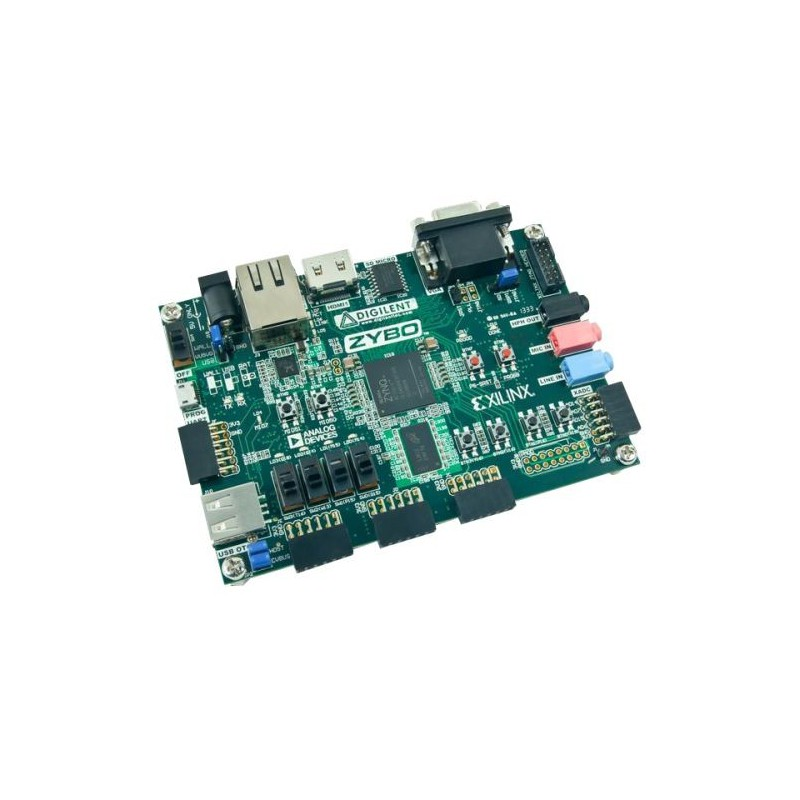
\includegraphics[width=4in]{zybo.jpg}
	%\caption{\label{fig:zybo}Płytka ZYBO Zynq-7000.}
	\captionsource{Płytka ZYBO Zynq-7000.}{\cite{Xi}}
\end{figure}

Zdecydowano, że platformę obliczeniową stanowić będzie płytka ZYBO. Jest to bogato wyposażone narzędzie zawierające układ programowalny z rodziny Xilinx Zynq-7000. Układ ten oparty jest na architekturze Xilinx All Programable System-on-Chip, w której zintegrowany został dwurdzeniowy procesor ARM Cortex-A9 i układ programowalny FPGA z serii Xilinx 7. Zawiera ona m.in. port HDMI potrzebne do odbieranie obrazu z kamery oraz port VGA, który umożliwia nam wysyłanie obrazu do monitora \cite{Xi}. W układzie programowalnym zaimplementowany zostanie tor wizyjny przetwarzający potokowo dane przesyłane z kamery oraz wyznaczający położenie obiektu w danej ramce. Oprócz tego musi on komunikować się ze sterownikiem serwomechanizmów w celu pozycjonowania głowicy w wyznaczonym punkcie oraz z komputerem klasy PC, aby otrzymywać parametry pracy oraz ustawiać początkową pozycję głowicy.

\section{Serwomechanizmy}
\label{sec:serwomechanizmy}

Ruchomą głowicę postanowiono skonstruować wykorzystując serwomechanizmy dostępne na rynku. Przy wyborze brano pod uwagę serwomechanizmy analogowe, serwomechanizmy cyfrowe oraz serwomechanizmy smart.

\subsection{Serwomechanizm analogowy}
Serwomechanizm ten sterowany jest impulsami podawanymi z częstotliwością 50 Hz. Podawanie impulsów z większą częstotliwością może doprowadzić do uszkodzenia urządzenia. W zależności od czasu trwania impulsu serwomechanizm ustawia się w odpowiedniej pozycji i ją utrzymuje. Kontrola położenia odbywa się za pomocą potencjometru sprzężonego z kołem zębatym. Serwomechanizm tego typu nie reagują szybko i nie produkują wystarczającego momentu kiedy zadajemy małe przesunięcie.

\subsection{Serwomechanizm cyfrowy}
Jest on, podobnie jak serwomechanizm analogowy, sterowany impulsami. Podawać można je jednak z maksymalną częstotliwością powyżej 300 Hz. W porównaniu do serwomechanizmu analogowego przyspiesza ono szybciej i produkuje stabilniejszy moment obrotowy. Reagują również lepiej na polecenia małych zmian pozycji. Z drugiej strony  potrzebują one dużo większej mocy. Prąd, który pobierają w trakcie pracy, może sięgać kilku amperów.

\subsection{Serwomechanizm smart}
Główną różnicą pomiędzy serwomechanizmami standardowymi, a smart, jest sposób komunikacji w celu podania wartości zadanej położenia. Zamiast impulsów o różnej szerokości wykorzystuje się komunikację szeregową. Ich obsługa jest więc bardziej skomplikowana. Najpopularniejszymi protokołami są TTL Half-Duplex, TTL Full-Duplex i RS-485. Za pomocą komunikacji tego typu można zmieniać dużo więcej parametrów niż tylko pozycję zadaną. Można zmieniać nastawy regulatora PID, maksymalną prędkość kątową lub maksymalny moment. W przeciwieństwie do serwomechanizmów klasycznych, możemy również odczytywać aktualną pozycję serwomechanizmu. Minusem tych urządzeń jest ich cena oraz dostępność. Są one kilka razy droższe od cyfrowych serwomechanizmów o podobnych parametrach.

\paragraph*{}
Postanowiono użyć dwóch serwomechanizmów cyfrowych PowerHD D-21HV. Są to serwomechanizmy typu standard o dużym momencie obrotowym i wysokiej maksymalnej prędkości obrotowej. Wyposażone jest w łożyska kulkowe oraz tytanowe tryby w celu zwiększenia jego wytrzymałości. Specyfikacja serwomechanizmów:
\begin{itemize}
\item Napięcie zasilania: \(6.0-7.4\) V
\item Zakres ruchu: \(155^\circ\)
\item Masa: \(75\) g
\item Moment: \(21\) kg\(\cdot\)cm dla napięcie \(7.4\) V
\item Prędkość: \(0.12\)s/\(60^\circ\) dla napięcia \(7.4\) V
\end{itemize}
\paragraph*{}
Urządzenia te mogą pobierać impulsowy prąd o wartości nawet powyżej 3 A. Sterowane są za pomocą impulsów podawanych z częstotliwością 333 Hz. Pozycję naturalną zadajemy podając impulsy o czasie trwania \(1500 \mu\)s. Serwa zostały połączone w głowicę za pomocą metalowych uchwytów dedykowanych do łączenia serwomechanizmów typu standard w konfigurację PT.

\section{Sterownik serwomechanizmów}
\label{sec:sterownik}

\begin{figure}[h]
	\centering
	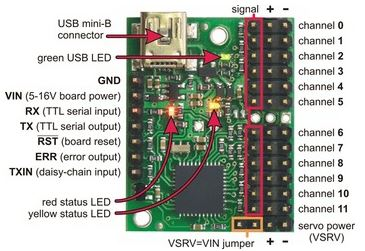
\includegraphics[width=4in]{maestro.jpg}
	\captionsource{Sterownik serwomechanizmów Pololu Mini Maestro.}{\cite{MM}}
\end{figure}

Do sterowania serwomechanizmami postanowiono użyć gotowego sterownika produkowanego przez firmę Pololu. 12-kanałowy sterownik Mini Maestro pozwala na równoczesną obsługę obu serwomechanizmów. Oprócz podawania wartości zadanej w postaci impulsów pozwala on również na zmianę ustawianie maksymalnej prędkości obrotowej i maksymalnego momentu obrotowego. Dzięki temu możemy dużo lepiej kontrolować urządzenia wykonawcze i zapewnić bardziej ciągły ruch głowicy. Komunikujemy się z nim za pośrednictwem interfejsu szeregowego UART z prędkością 115200 bitów na sekundę.

\section{Zasilanie}
\label{sec:zasilanie}
Do zasilania głowicy użyty został zasilacz impulsowy Redox, który na wyjściu daje napięcie 12 V i maksymalny prąd 5 A. Jako, że serwomechanizmy potrzebują napięcia 7.4 V używamy przetwornicy step-down XL4005E1 o regulowanym napięciu wyjściowym. Maksymalny prąd wyjściowy użytej przetwornicy wynosi 5 A. Zdecydowanie wystarczy to do zasilenia użytych serwomechanizmów.

\section{Wskaźnik}
\label{sec:wskaznik}

Postanowiono użyć zwykłego wskaźnika laserowego do wskazywania miejsca, w stronę którego zwrócona jest głowica.
\chapter{Komunikacja}
\label{cha:komunikacja}

Po zbudowaniu stanowiska postanowiono w pierwszej kolejności zaimplementować komunikację między wszystkimi elementami systemu. 
Można ją podzielić na część PC-Zynq oraz Zynq-sterownik serwomechanizmów "Maestro".
%TODO Maestro - niesjane... -zrobione.

\section{PC-Zynq}
\label{sec:pc-zynq}
Postanowiono wykorzystać UART. 
Argumentem przemawiającym za tym rozwiązaniem był fakt wyprowadzenia dwóch pinów MIO (48 i 49) procesora karty ZYBO do złącza mikro USB typu B. 
Piny te podłączone zostały do jednego z układów procesora odpowiedzialnych za komunikację szeregową - UART1. 
Złącze USB służy również do programowania układu przez JTAG.
Dzięki temu używa się jednego przewodu do programowania układu oraz do komunikacji z nim. 
Po podłączeniu przewodu oraz włączeniu ZYBO w komputerze pojawia się dodatkowy port COM. 
Przez ten port można wymieniać dane z platformą obliczeniową. Do wysyłania komunikatów na PC wykorzystano program \textit{Realterm}. 
Dzięki temu nie było konieczności pisania dodatkowego oprogramowania. Okno programu \textit{Realterm} zostało przedstawione na rysunku \ref{fig:realterm}.

\begin{figure}[h]
	\centering
	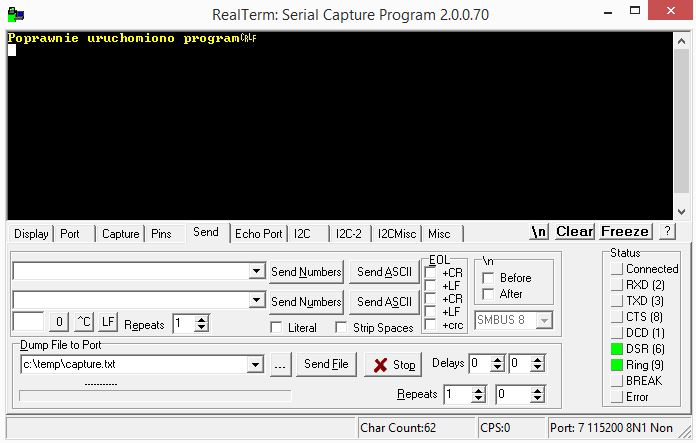
\includegraphics[width=4in]{realterm.jpg}
	\caption{Okno programu Realterm z komunikatem o poprawnym uruchomieniu programu.}
	\label{fig:realterm}
\end{figure}

\paragraph*{}
Rozmiar jednej komendy wysyłanej do układu Zynq wynosi 5 bajtów.
Pierwszy informuje o typie rozkazu, a 4 kolejne są danymi do tego rozkazu.
Każdy kolejny odebrany bajt umieszczany jest w buforze o rozmiarze 5 bajtów.
Włączone zostało przerwanie od pełnego bufora.
Po wysłaniu komendy z PC w procesorze układu Zynq uruchamiane jest przerwanie, w którym wysłany zostaje odpowiedni rozkaz do sterownika serwomechanizmów lub ustawiana jest zmienna informująca o pracy w trybie autonomicznym, podczas którego kamera ustawiana jest tak, by obiekt znajdował się w centrum kadru.
%TODO niejasne, bo wczesniej tryb autonomiczny sie nie pojawił. -zrobione.
Zaimplementowano obsługę następujących komend w Zynq:
\begin{itemize}
\item Zmiana pozycji serwomechanizmów: 0x00 0xHH 0xLL 0xHH 0xLL.
\item Zmiana maksymalnej prędkości serwomechanizmów: 0x01 0xHH 0xLL 0xHH 0xLL.
\item Zmiana maksymalnego momentu serwomechanizmów: 0x02 0xHH 0xLL 0xHH 0xLL.
\item Odczyt aktualnej wartości zadanej ze sterownika: 0x03 0x-- 0x-- 0x-- 0x--.
\item Rozpoczęcie pracy autonomicznej (śledzenia): 0x04 0x-- 0x-- 0x-- 0x--.
\end{itemize}
\paragraph*{}
W pierwszych trzech rozkazach pierwsze dwa bajty danych są parametrami dla serwomechanizmu odpowiedzialnego za obrót, a kolejne dwa są parametrami dla serwomechanizmu odpowiedzialnego za nachylenie. 
Myślniki w kolejnych komendach oznaczają, że wysłane bajty danych nie są istotne (komendy te nie potrzebują danych).

\section{Zynq-Maestro}
\label{sec:zynq-maestro}

% Tutaj wstaw zdjęcie połączonego układu ZYBO-Maestro.

Komunikacja przez UART została narzucona, gdyż jest to jedyny protokół komunikacyjny w Maestro. 
Połączone zostały odpowiednie piny (MIO 14,15) złącza MIO PMOD karty ZYBO do pinów Maestro odpowiadających za komunikację szeregową.
Następnie do użytych pinów MIO podłączono wyjścia innego układu procesora odpowiadającego za komunikację szeregową - UART0.
W dokumentacji Maestro wyszukano listę komend i zaimplementowano wysyłanie potrzebnych w układzie Zynq \cite{MM}. Są to następujące komendy:
\begin{itemize}
\item Zmiana pozycji serwomechanizmów: 0x9F 0x02 0x0A 0xLL 0xHH 0xLL 0xHH.
\item Zmiana maksymalnej prędkości serwomechanizmów: 0x87 0x0A/0x0B 0xLL 0xHH.
\item Zmiana maksymalnego momentu serwomechanizmów: 0x89 0x0A/0x0B 0xLL 0xHH.
\item Odczyt pozycji ze sterownika: 0x90 0x0A/0x0B.
\end{itemize}
W powyższych komendach A oznacza obrót, a B nachylenie (są to numery kanałów sterownika zapisane szesnastkowo).

\section{Testy komunikacji}
\label{testy_komunikacji}
Komunikacja była testowana na układzie złożonym z:
\begin{itemize}
\item Komputera klasy PC.
\item Karty ewaluacyjnej ZYBO.
\item Komputera Raspberry Pi 2 Model B.
\end{itemize}
Karta ZYBO połączona wraz z połączonym komputerem Raspberry Pi 2 B zostały przedstawione na rysunku \ref{fig:raspberry}.

\begin{figure}[h]
	\centering
	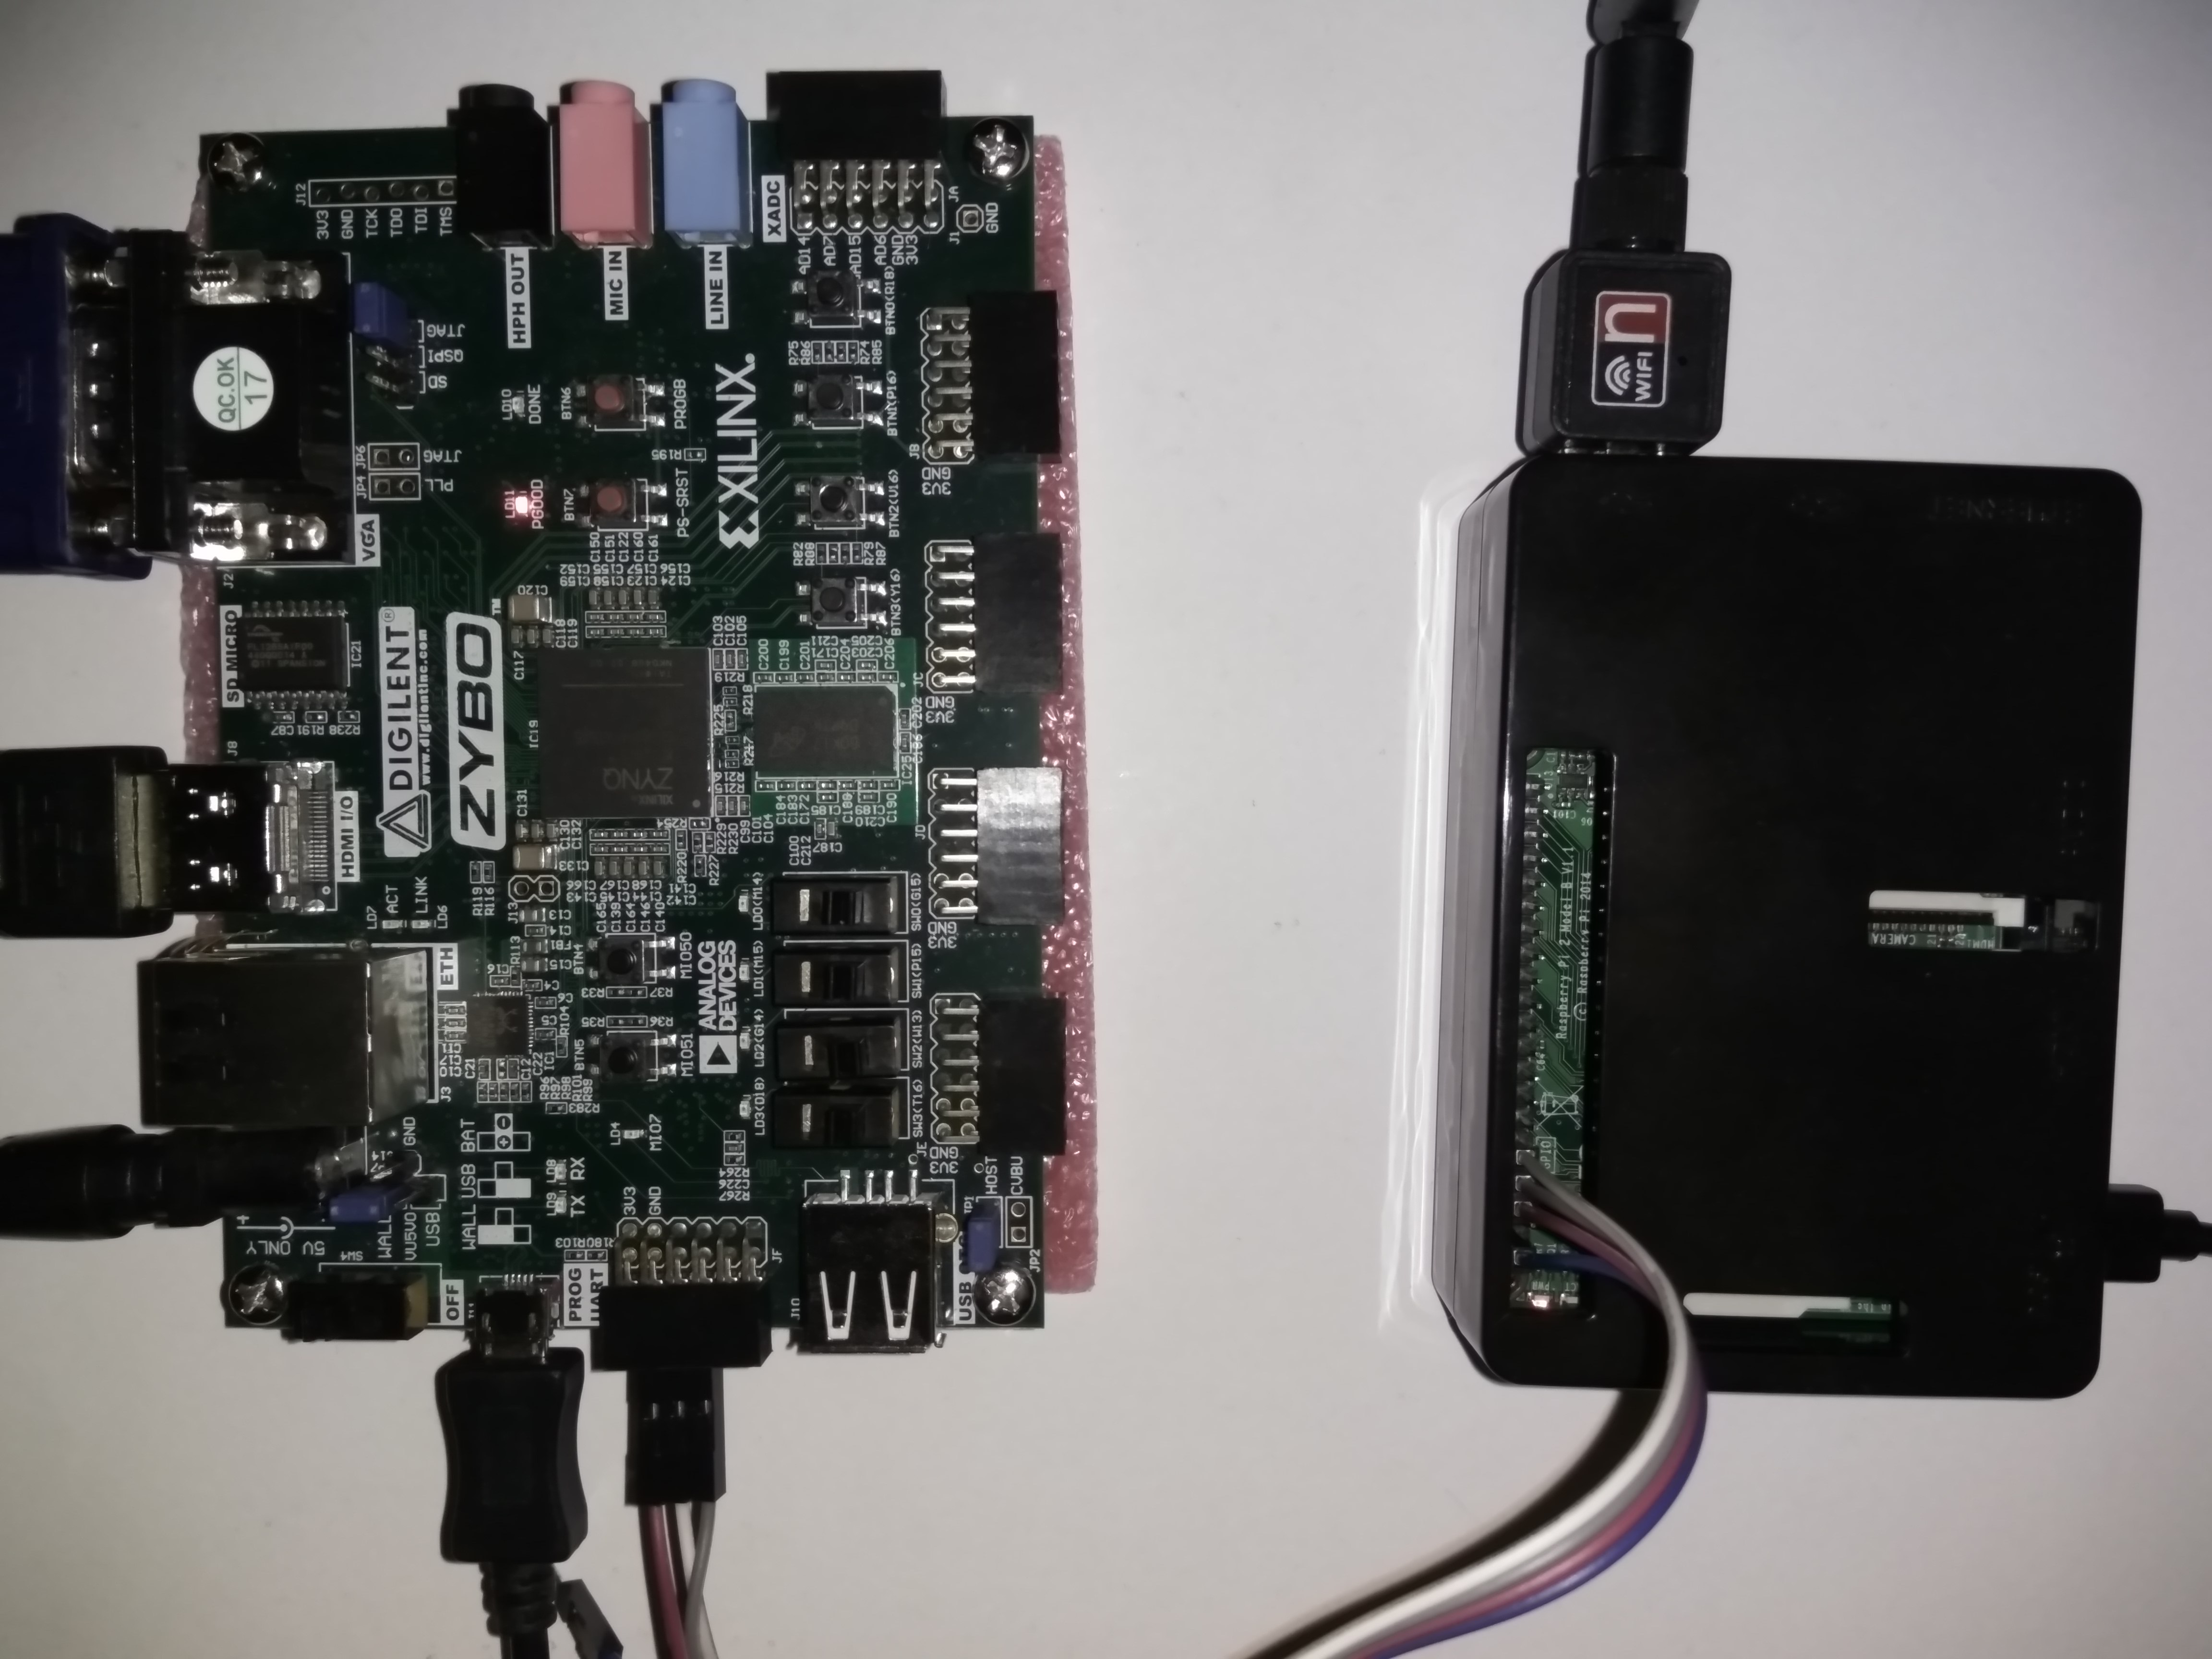
\includegraphics[width=4in]{raspberry.jpg}
	\caption{Karta ewaluacyjna ZYBO i komputer Raspberry pi 2 B użyty do testów.}
	\label{fig:raspberry}
\end{figure}

\paragraph*{}
W układzie tym Raspberry zastępowało sterownik serwomechanizmów.
Zamiana ta została wykonana, by mieć możliwość sprawdzania poprawności danych odbieranych z Zynq.
W trakcie testów okazało się, że pierwszy bajt wysyłany do ZYBO jest wpisywany do bufora i wskaźnik jest przesuwany, lecz w kontrolerze przerwań nie jest zwiększany licznik liczby bajtów w buforze.
W efekcie przerwanie od pełnego bufora danych przychodzących było wywoływane o 1 bajt za późno (po otrzymaniu pierwszego bajtu nowej komendy).
Naprawiono to poprzez dodatkowy test w trakcie inicjalizacji komunikacji szeregowej.
Polegał on na włączeniu trybu \textit{loopback}, wysłaniu i odebraniu kilku bajtów danych, a następnie zresetowaniu bufora. W trybie \textit{loopback} dane wysyłane przez UART są wysyłane na jego wejście.
W ten sposób można sprawdzać zgodność danych.
Oprócz tego sprawdzono, czy wysłanie komendy z PC do Zynq skutkuje wysłaniem poprawnej komendy z Zynq do Maestro.
Po naprawieniu opisanego problemu i ponownym przeprowadzeniu testów stwierdzono, że komunikacja działa poprawnie.


% itd.
% \appendix
% \chapter{Zawartość płyty CD}
\label{cha:zawartoscplytycd}

Na załączonej płycie CD znajduje się:
\begin{itemize}
\item Tekst pracy w formacie PDF.
\item Projekt Vivado systemu z algorytmem śledzenia przez detekcję.
\item Projekt Vivado systemu z algorytmem Mean-shift.
\item Projekt Vivado z algorytmem wykrywania punktów charakterystycznych.
\item Kod \textit{MATLAB} użyty do oceny algorytmów śledzenia.
\end{itemize}
% \include{dodatekB}
% itd.

\printbibliography

\end{document}